\chapter{UNIX システムを使ってみよう}

\section{システムの起動、終了、ログイン、ログアウト}

\subsection{システムの起動}

 B 演習室の PC/AT 互換機には、 Windows XP と Windows NT と FreeBSD が入っている。
 FreeBSD を起動するには次のようにする。

\begin{enumerate}
\item 電源スイッチをいれる。
\item OS Loader が起動し、次の図のようになるので、 FreeBSD を選択し、
 \KEYTOP{Enter} を押す。
\begin{figure}[H]
\centering{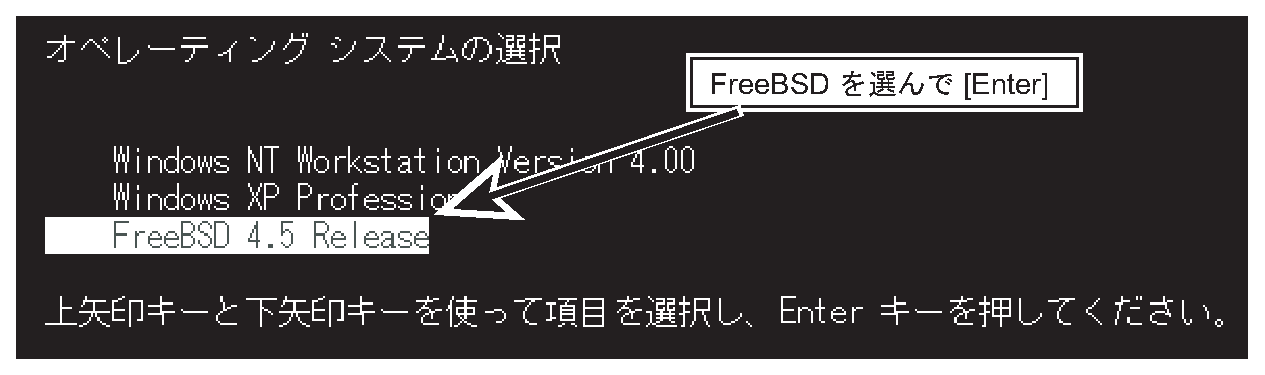
\includegraphics[scale=0.7]{bootloader.eps}}
\end{figure}
\item 「\texttt{Booting [kernel] in ○ seconds...}」と表示されるので、 \KEYTOP{Enter} を押す(下の図では \KEYTOP{Enter} を \retrn と書いている)。
これは放っておいても大丈夫である。
\begin{progls}
BTX loader 1.00 BTX version is 1.01
Console: internal video/keyboard
BIOS drive A: is disk0
BIOS drive C: is disk1
BIOS 639kB/392064KB available memory
                                   \vdots
                                 \fbox{中略}
                                   \vdots
Hit [Enter] to boot immediately, or any other key for command prompt.
Booting [kernel] in 6 seconds... _\retrn
\end{progls}
\item FreeBSD が起動し、 X Window System が立ち上がる。
そして、次の図のように XDM\footnote{X Display Manager} の login 画面になる。
\begin{figure}[H]
\centering{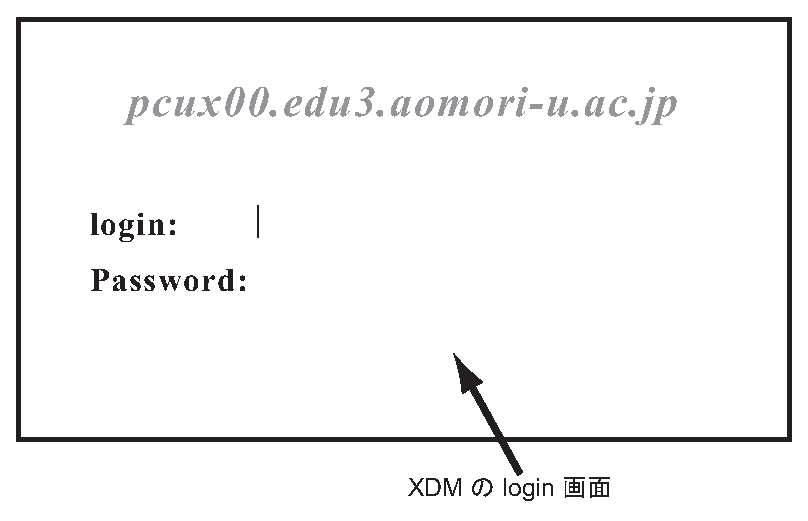
\includegraphics[scale=0.7]{xdm01.eps}}
\end{figure}
\end{enumerate}

以上で、起動は OK である。

\subsection{ログイン}

\subsubsection{ID とパスワードがまず必要}

 UNIX システムを使うためには、そのシステムの管理者が用意してくれた
 ID とパスワードが必要になる。

\bigskip

 ID は UNIX システムを使うときのユーザの名前である。
これは、そのシステムを使うときにずっと使うもので、
ユーザが自分で勝手に変えることはできない。
 ID には、例えば \texttt{kokubo}、 \texttt{judy}、 \texttt{aichan}、
 \texttt{rms} のように、名前やニックネーム、頭文字を使ったりすることもある。
また、 \texttt{ei00001}、 \texttt{0198011}、 \texttt{tz0la92} のように、
学校の学籍番号や、会社の社員番号や、ランダムな文字列を使うこともある。

\bigskip

パスワードは、たぶんシステムの管理者が用意してくれたものを最初に渡されるだろう。
これをユーザは、自分で好きなものに変更して使う。
パスワードの変更の仕方は後の方で説明する。

\newpage

\subsubsection{XDM からのログイン}

B 演習室のマシンは、 UNIX システムが起動すると、 XDM のログイン画面がでる。
この画面からログインするには、次のようにする。

\begin{enumerate}
\item 「login:」のところに ID を入力して、 \KEYTOP{Enter}。
\item 「Password:」のところにパスワードを入力して(打った文字は見えない)、 \KEYTOP{Enter}。
\begin{figure}[H]
\centering{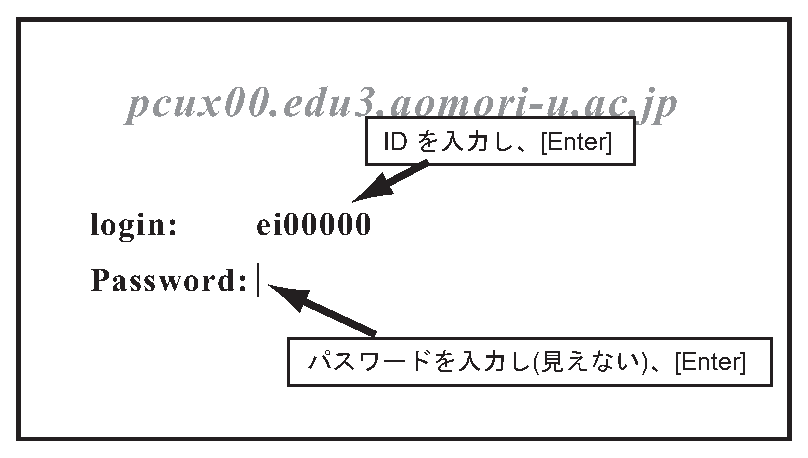
\includegraphics[scale=0.7]{xdm02.eps}}
\end{figure}
\item login に成功すると、次のような画面になる。
失敗した場合は、赤字で「Login incorrect」と表示されるので、
 ID を入力するところからやりなおす。
\begin{figure}[H]
\centering{\includegraphics[scale=0.5]{logsuc.eps}}
\end{figure}
\end{enumerate}

\newpage

\subsection{ログアウト}

UNIX システムからログアウトする方法を説明しよう。

\begin{enumerate}
\item 起動しているプログラムを一通り終了する(終了の仕方は後で説明する)。
\item 画面の何もない部分で、左ボタンをクリックする。
\item 「Twm」と書かれたメニューが出るので、左ボタンを押したまま、
 1 番下の「Exit」までマウスを移動してから、指をはなす。
\begin{figure}[H]
\centering{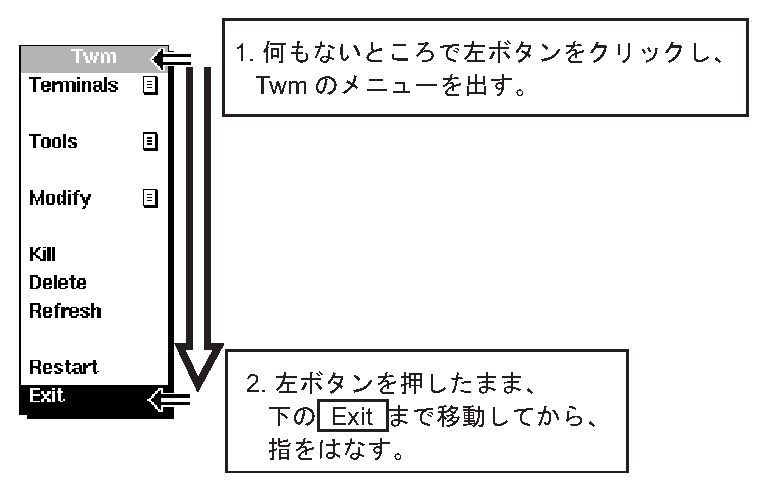
\includegraphics[scale=0.7]{twmmenu01.eps}}
\end{figure}
\item XDM の login 画面になって、ログアウトが完了する。
\end{enumerate}

\newpage

\subsection{システムの終了}

通常、 UNIX システムは、電源を切らないで 24 時間動かしっぱなしに
することが多い。
また、普通のユーザは電源を切ることができず、システム管理者だけが
これを行うことができる。

しかし、B 演習室のマシンは、 Windows に切替えて使ったりするために、
普通のユーザでも電源を切ることができるように設定されている。
ちなみに、ここに書かれているように実行しても、 B 演習室以外のマシンでは
終了できないので、注意すること。

では、電源の切り方を説明しよう。
この手順通りに実行しないと、システムがクラッシュしたりする可能性が
あるので注意すること。

\begin{enumerate}
\item UNIX システムを使っている場合は、ログアウトして、 XDM の login 画面にする。
\item login: に対して、「shutdown」と入力して \KEYTOP{Enter} する。
\item Password: に対して、何も入力しないで \KEYTOP{Enter} する。
\begin{figure}[H]
\centering{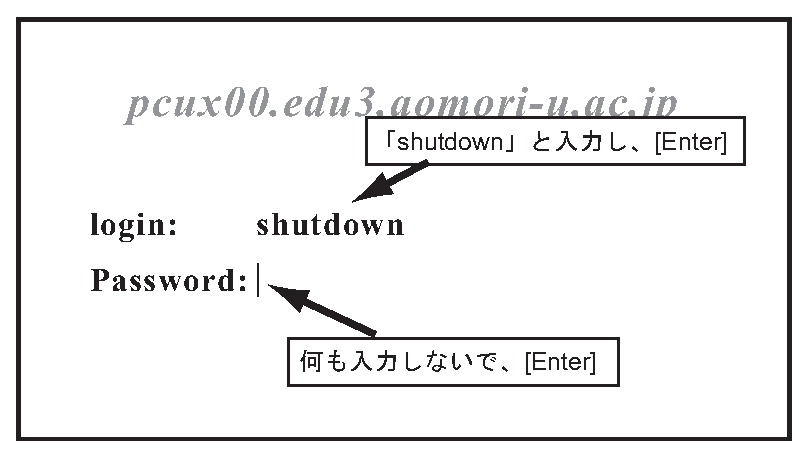
\includegraphics[scale=0.7]{xdm03.eps}}
\end{figure}
\item 一瞬、間をおいて shutdown が実行される。
\item 次のようなメッセージがでて、システムが終了する。
\begin{progls}
  The operating system halted. (オペレーティング・システムは停止しました。)
  Please press any key to reboot. (再起動するには何かキーを押してください。)
\end{progls}
\item 今回は\underline{再起動しない}ので、\underline{何もキーを押さず}に、
電源スイッチを押して、電源を切る。
\end{enumerate}

\newpage

\section{パスワードの変更}

最初、システム管理者からパスワードが配られると思うが、 UNIX システムでは
自分で好きなパスワードに変更できる。
ここでは、その方法を紹介しよう。

\subsection{パスワードの条件}

まず、 FreeBSD の場合、パスワードには次のような条件がある。

\begin{coml}{14cm}
\begin{normalsize}
\begin{enumerate}
\item 文字数は 6 〜 128文字
\item 使える文字は、英、数、記号
\item ただし、大文字だけ、小文字だけのパスワードはダメ。
\end{enumerate}
\end{normalsize}
\end{coml}

\subsection{どんなパスワードがいいか}

では、どんなパスワードがいいかというと次のようなものだ。
\begin{enumerate}
\item 万一、一瞬他人から見られても、何だかよくわからないもの。
\item 自分では忘れにくい。
\item 大、小文字、数字、記号などが適当に混じっている。
\end{enumerate}

逆に危険なパスワードは、次のようなものだ。

\begin{enumerate}
\item 辞書にそのまま載っているような単語。
\item 自分の名前、電話番号、住所など、他人から簡単に想像できるものを
\underline{そのまま}使う。
\item あまりに長いなど、自分でも覚えられないようなもの。
\end{enumerate}

\subsection{パスワードの変更}

パスワードを決めたら、変更することにする。
変更するには、次のようにする。

\begin{enumerate}
\item マウスをウィンドウに入れる。
\item 「\texttt{passwd}」と入力し、 \KEYTOP{Enter}。
\item 「Old Password:」に対して、現在のパスワードを入力し、 \KEYTOP{Enter}
\item 「New password:」に対して、新しいパスワードを入力し、 \KEYTOP{Enter}
\item 「Retype new password:」に対して、もう一度新しいパスワードを入力し、
 \KEYTOP{Enter}
\item 「NIS password has been changed on uxsv1.edu3.aomori-u.ac.jp.」と出れば、
変更に成功。
だめなら、 2 番からやり直す。
\end{enumerate}
\begin{figure}[H]
\centering{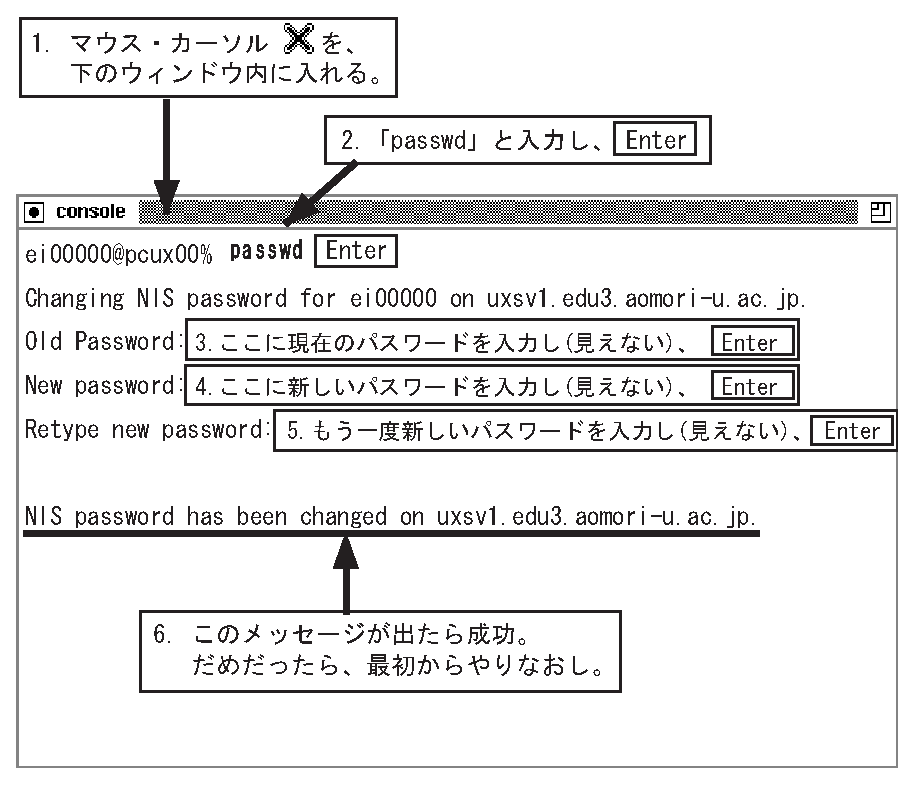
\includegraphics[scale=0.7]{passwd.eps}}
\end{figure}

\subsubsection{パスワードの変更に失敗したときのエラー・メッセージ}

パスワードの変更に失敗すると、次のようなエラー・メッセージが出る。
その意味を説明しよう。

\begin{enumerate}
\item 「\textbf{password: Sorry.}」

→ 現在のパスワードが間違っていた。
\item 「\textbf{Please enter a password at least 6 characters in length}」

→ 新しいパスワードが短すぎた(最低でも 6 文字以上)。
\item 「\textbf{Please don't use an all-lower case password.
Unusual capitalization, control charactors or digits are suggested.}」

→ パスワードが全部小文字だった。
\item 「\textbf{Mismatch: try again, EOF to quit.}」

→ 新しいパスワードとして入力したものが 1 回目と 2 回目で異なっていた。
\end{enumerate}

\newpage

\section{X Window System 入門}

ここでは、 X Window System について、簡単に紹介する。
 X Windows System の操作は実際にはウィンドウ・マネージャの種類に
よって異なってくるが、ここでは従来から標準的に用いられている Twm を
取り上げることにする。

\subsection{マウスのボタンの呼び方}

まず、最初にマウスのボタンの呼び方を紹介しよう。
 X Window System を使う UNIX では、普通、 3 つボタン・マウスを使う。
それぞれのボタンは、左から順番に、ボタン 1、 2、 3 と呼ぶ。

なお、 2 つボタン・マウスを使っているときは、
左右のボタンを同時に押すと、ボタン 2 の代わりになる\footnote{システム
管理者がそのように設定しておく必要がある。}。

\begin{figure}[H]
\centering{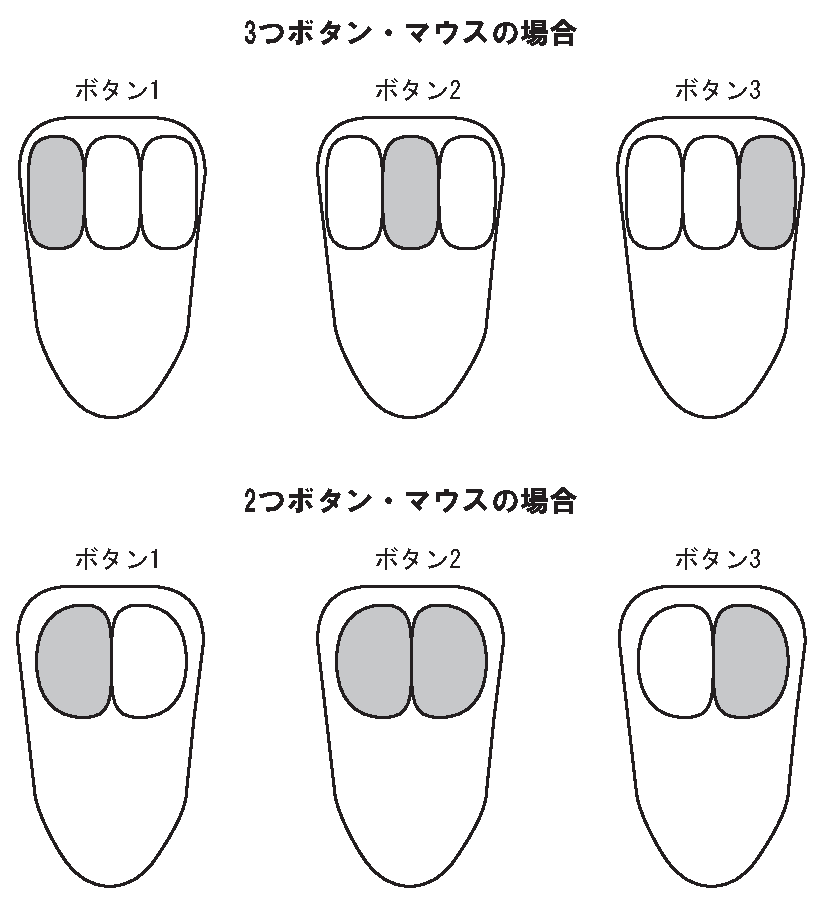
\includegraphics[scale=0.7]{mousebutton.eps}}
\end{figure}
\newpage

\subsection{画面内の各部の名称}

X Window System のデスクトップの名称を紹介しよう。
次の図のように、画面の背景を「ルート・ウィンドウ」、
画面の中に開かれている様々なプログラムを「ウィンドウ」と言う。
いくつかの「ウィンドウ」は、マウス・カーソルを入れると、文字を入力できる
ようになったりする。

\begin{figure}[H]
\centering{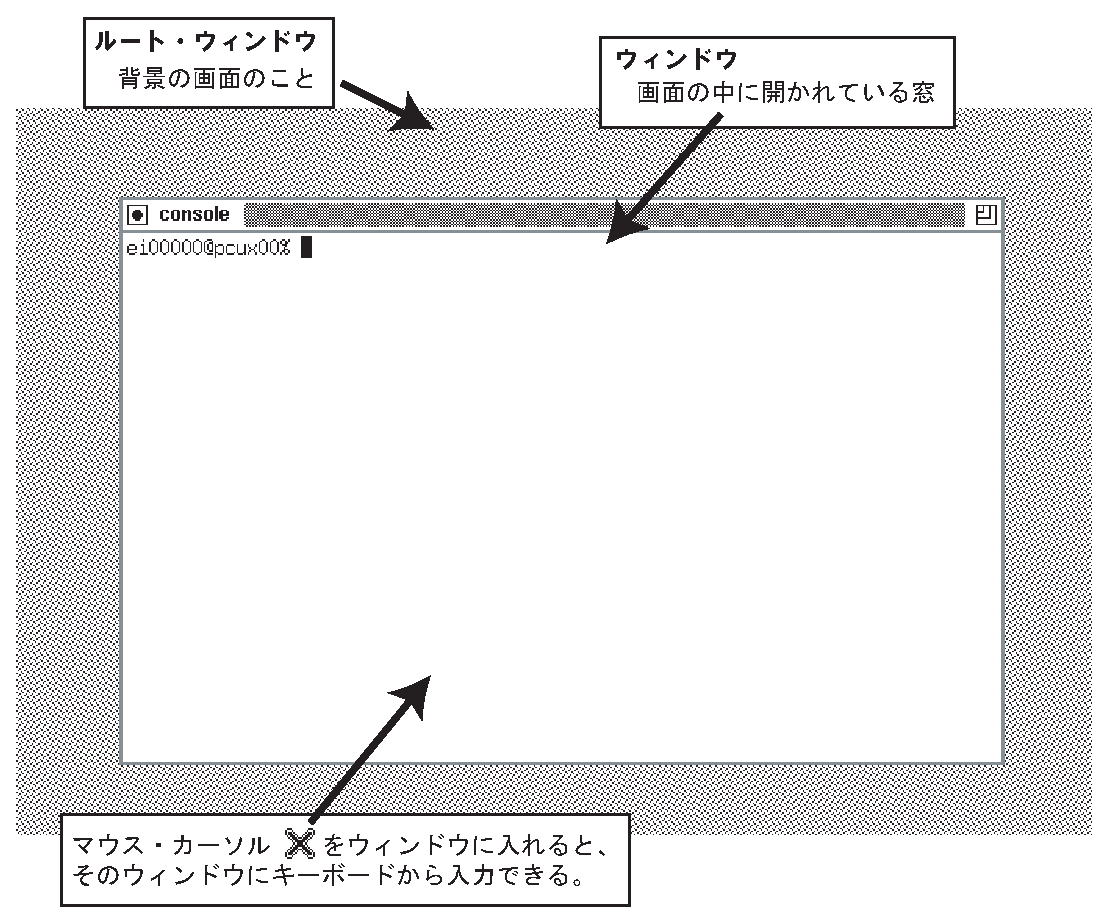
\includegraphics[scale=0.7]{rootwin.eps}}
\end{figure}

また、各ウィンドウの上部には、「バー」が付いている。
「バー」には、
持つとウィンドウを移動できる「タイトル・バー」、
クリックするとウィンドウがアイコン化される「アイコン化ボックス」、
ドラッグするとウィンドウのサイズを変更できる「リサイズ・ボックス」
などが付いている。

\begin{figure}[H]
\centering{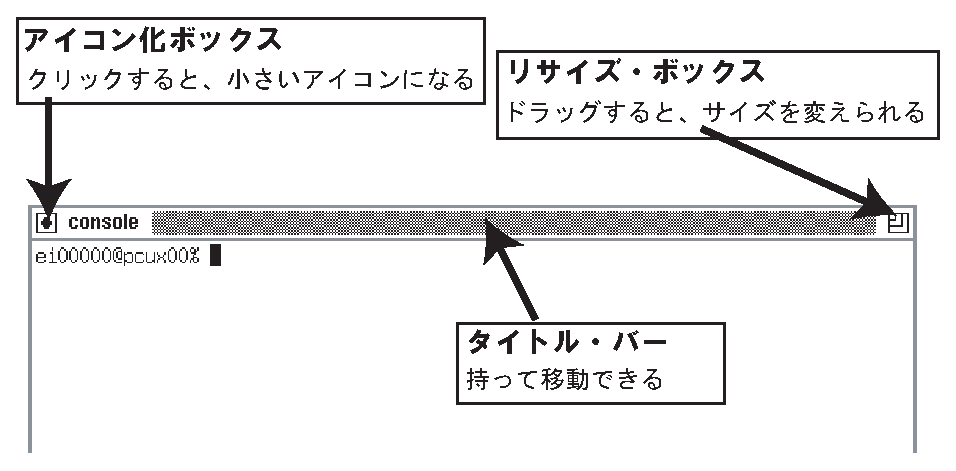
\includegraphics[scale=0.7]{win01.eps}}
\end{figure}

\newpage

\subsection{ウィンドウを開く}

ウィンドウを開く方法はいくつかある。
その代表的な方法を紹介しよう。

\subsubsection{ウィンドウを開くコマンドを入力}

まず、文字の入力できるウィンドウにマウス・カーソルを移動する。
そして、「\textbf{コマンド名} \texttt{\&}\retrn」と入力する。

では実際に、次のコマンドを、いくつか実行してみよう。

\bigskip

\noindent
\begin{minipage}[t]{20zw}
\begin{itemize}
\item \texttt{kterm \&}\retrn
\item \texttt{xeyes \&}\retrn
\item \texttt{xcalc \&}\retrn
\item \texttt{xclock \&}\retrn
\item \texttt{asclock \&}\retrn
\item \texttt{xengine \&}\retrn
\end{itemize}
\end{minipage}
\begin{minipage}[t]{20zw}
\begin{itemize}
\item \texttt{tksol \&}\retrn
\item \texttt{xmine \&}\retrn
\item \texttt{xbill \&}\retrn
\item \texttt{oneko \&}\retrn
\item \texttt{xearth \&}\retrn
\item \texttt{xsoldier \&}\retrn
\end{itemize}
\end{minipage}

\subsubsection{\texttt{\&}を最後に付け忘れると}

コマンドの最後に「\texttt{\&}」を付けずに実行すると、
元のウィンドウにタイプしても何も効かなくなる。

\begin{progls}
% \slbfl{kterm}\retrn
(ここにコマンドを入力しても何も効かない)
\end{progls}

このような場合は、まず「\KEYTOP{Ctrl}+z」と入力し
(入力すると「\verb+^Z+」と表示される)、
それ続けて「\texttt{bg}\retrn」と入力する。
すると、再び入力を受け付けるようになる。

\begin{progls}
% \slbfl{kterm}\retrn
\slbfl{^Z}
[1]+  Stopped                 kterm
% \slbfl{bg}\retrn
[1]+ kterm &
% (普通にコマンドが打てるようになる)
\end{progls}

\subsubsection{ウィンドウ・マネージャのメニューから選択}

ルート・ウィンドウでマウスの\KEYTOP{ボタン 1}をクリックするとメニューが出る。
このメニューからウィンドウを開くこともできる。

では実際に、次のようにしてみよう。

\begin{enumerate}
\item \KEYTOP{ボタン 1}を何もないところでクリックし、Twmのメニューを出す。
\item \KEYTOP{ボタン 1}を押したまま、「Terminals」まで移動し、少し右に移動する。
\begin{figure}[H]
\centering{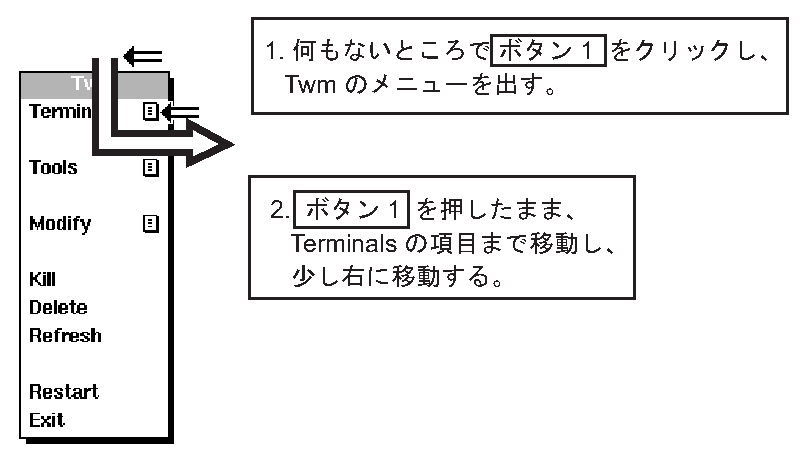
\includegraphics[scale=0.7]{twmmenu02.eps}}
\end{figure}
\item 新たにメニューが出る。
\item 「Kterm」まで移動して、指をはなす。
\begin{figure}[H]
\centering{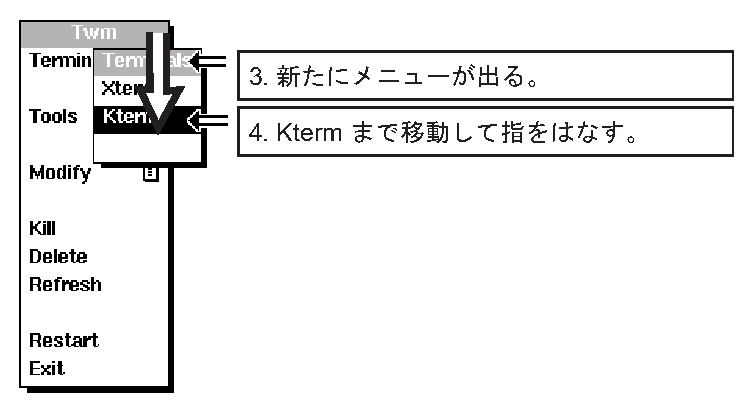
\includegraphics[scale=0.7]{twmmenu03.eps}}
\end{figure}
\smallskip
\item マウスで確定してやると、Kterm が起動してウィンドウが開く。
\begin{figure}[H]
\centering{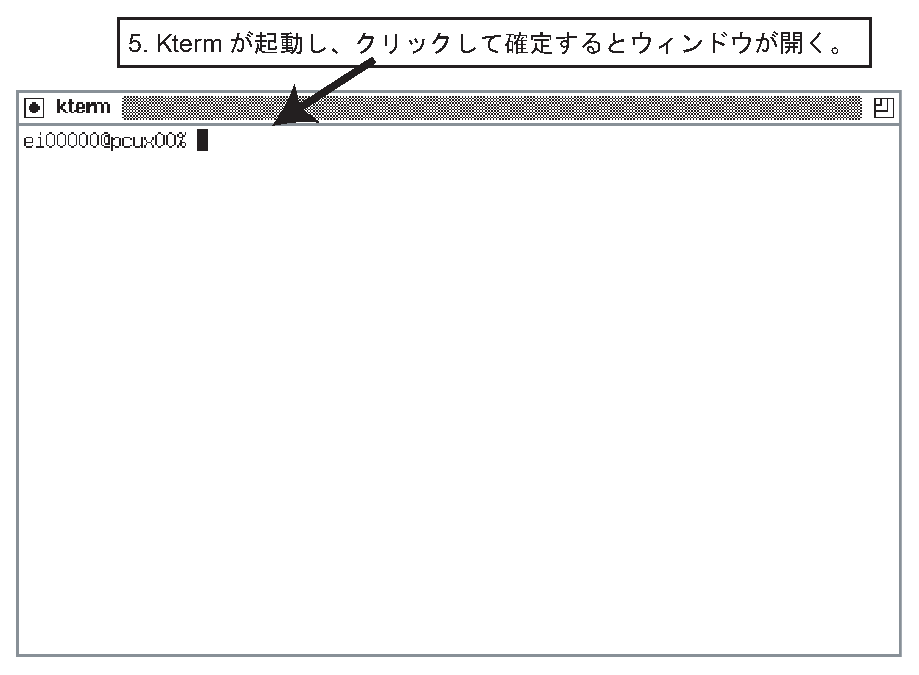
\includegraphics[scale=0.7]{twmmenu04.eps}}
\end{figure}
\end{enumerate}

\subsection{ウィンドウを閉じる}

ウィンドウを閉じる方法も何種類かある。

\subsubsection{\texttt{exit}コマンドを入力}

Kterm のように、コマンドが入力できるウィンドウを閉じる場合は、
「\texttt{exit}」と入力する。

\begin{progls}
ei00000@pcux00% \slbfl{exit}\retrn
\end{progls}

\subsubsection{ウィンドウのメニューから exit などを選ぶ}

いくつかのウィンドウには、メニューが付いている。
このメニューの「file」などの項目から、「exit」などを選ぶと終了できる。

\subsubsection{ウィンドウ・マネージャのメニューから「Delete」を選ぶ}

上の 2 つの方法で終了できない場合は、Twmのメニューから「Delete」を
選ぶと「終了」させられる。
なお、「Kill」を選んだ場合は、「強制終了」になる。

\begin{enumerate}
\item 何もないところでクリックし、「Twm」のメニューを出す。
\item クリックしたまま「Delete」まで移動し、指をはなす。
\item ドクロに変わったマウス・カーソルで、閉じたいウィンドウをクリックする。
\end{enumerate}

\begin{figure}[H]
\centering{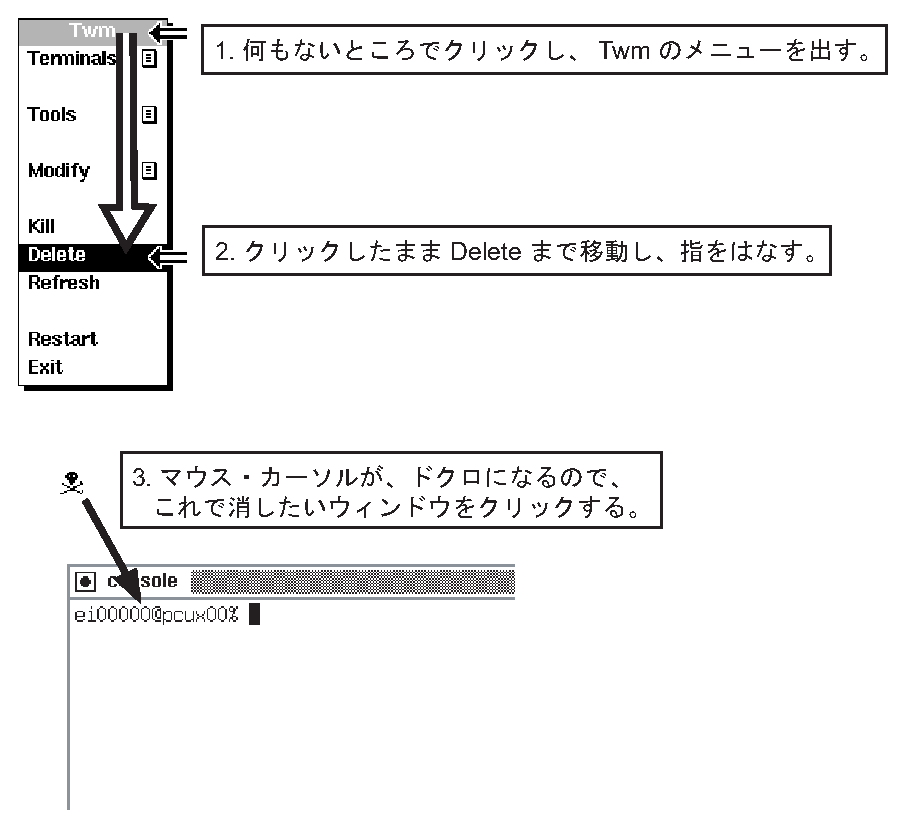
\includegraphics[scale=0.7]{delete.eps}}
\end{figure}

\subsection{ウィンドウのアイコン化}

アイコン化ボックスをクリックすると、ウィンドウがアイコン(小さいマーク)化される。
元に戻すには、アイコンをクリックすればよい。

\begin{figure}[H]
\centering{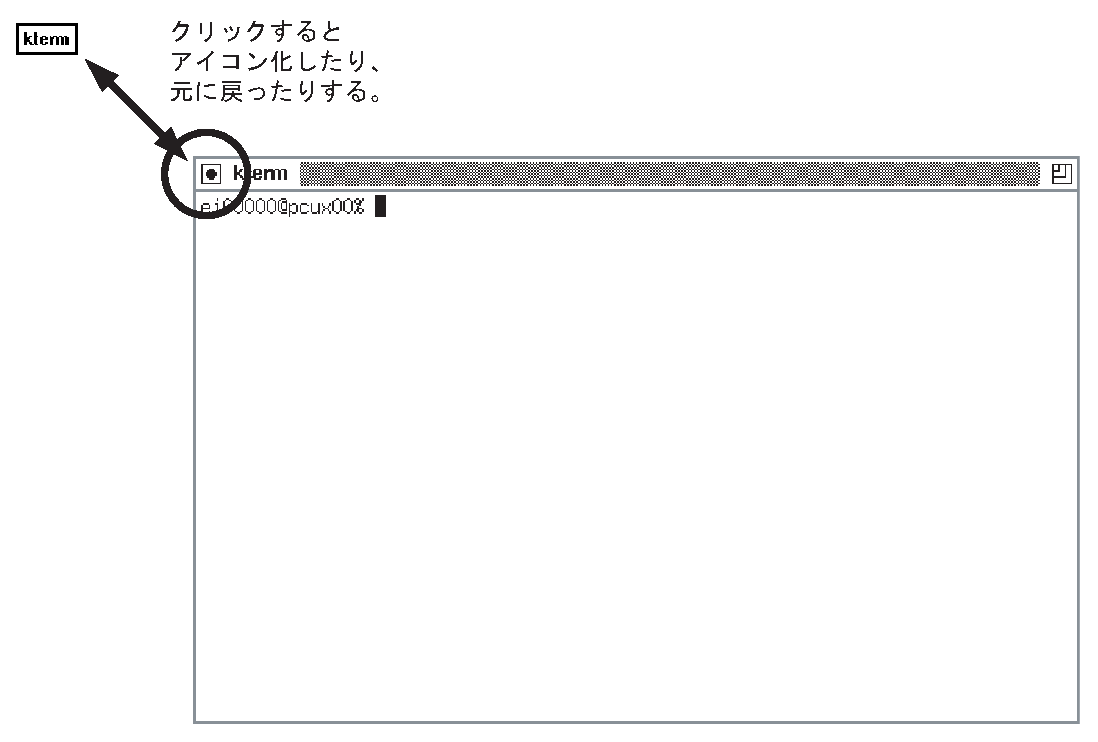
\includegraphics[scale=0.7]{iconize.eps}}
\end{figure}

%\newpage

\subsection{ウィンドウの移動}

ウィンドウのタイトル・バーを持てば、ウィンドウを移動することができる。

\begin{figure}[H]
\centering{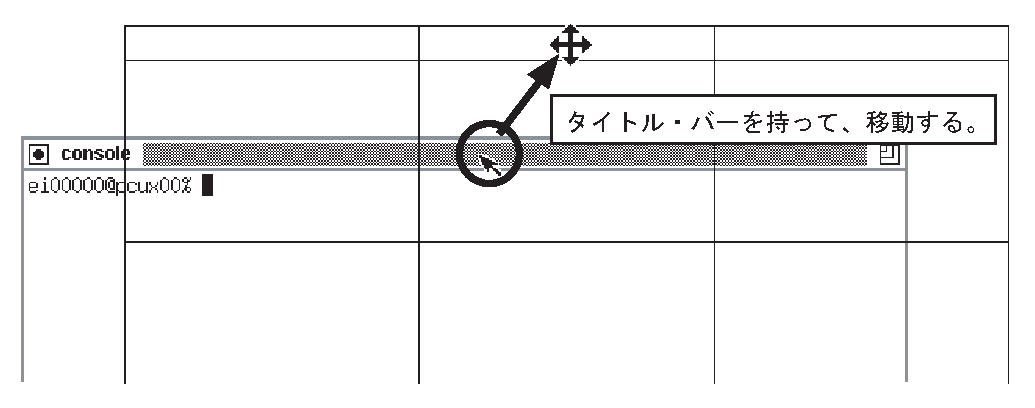
\includegraphics[scale=0.7]{move.eps}}
\end{figure}

\subsection{ウィンドウの大きさの変更}

ウィンドウの大きさは、「リサイズ・ボックス」を持って、
ドラッグすることで変更できる。

\begin{enumerate}
\item 大きくするとき

単にリサイズ・ボックスをクリックし、そのままドラッグして広げる。
\item 小さくするとき

大きくするときと同様だが、一旦、少しだけ広げてからでないと、小さくできない。
\end{enumerate}

\begin{figure}[H]
\centering{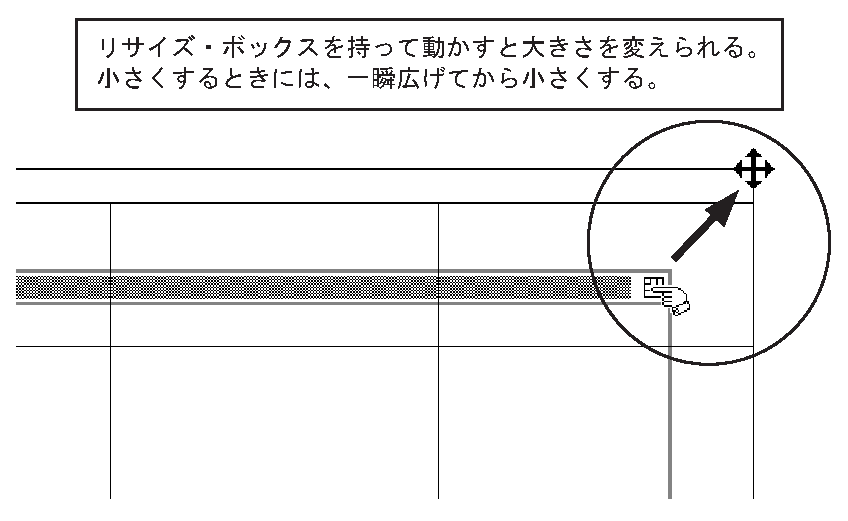
\includegraphics[scale=0.7]{resize.eps}}
\end{figure}

%\newpage

\subsection{重なったウィンドウを一番上にする}

重なったウィンドウを上にする方法は何通りかある。
ここでは、いくつか紹介しよう。

\subsubsection{上にしたいウィンドウのタイトル・バーをクリック}

下になっているウィンドウのタイトル・バーをクリックすると、一番上に出すことが
できる。

\begin{figure}[H]
\centering{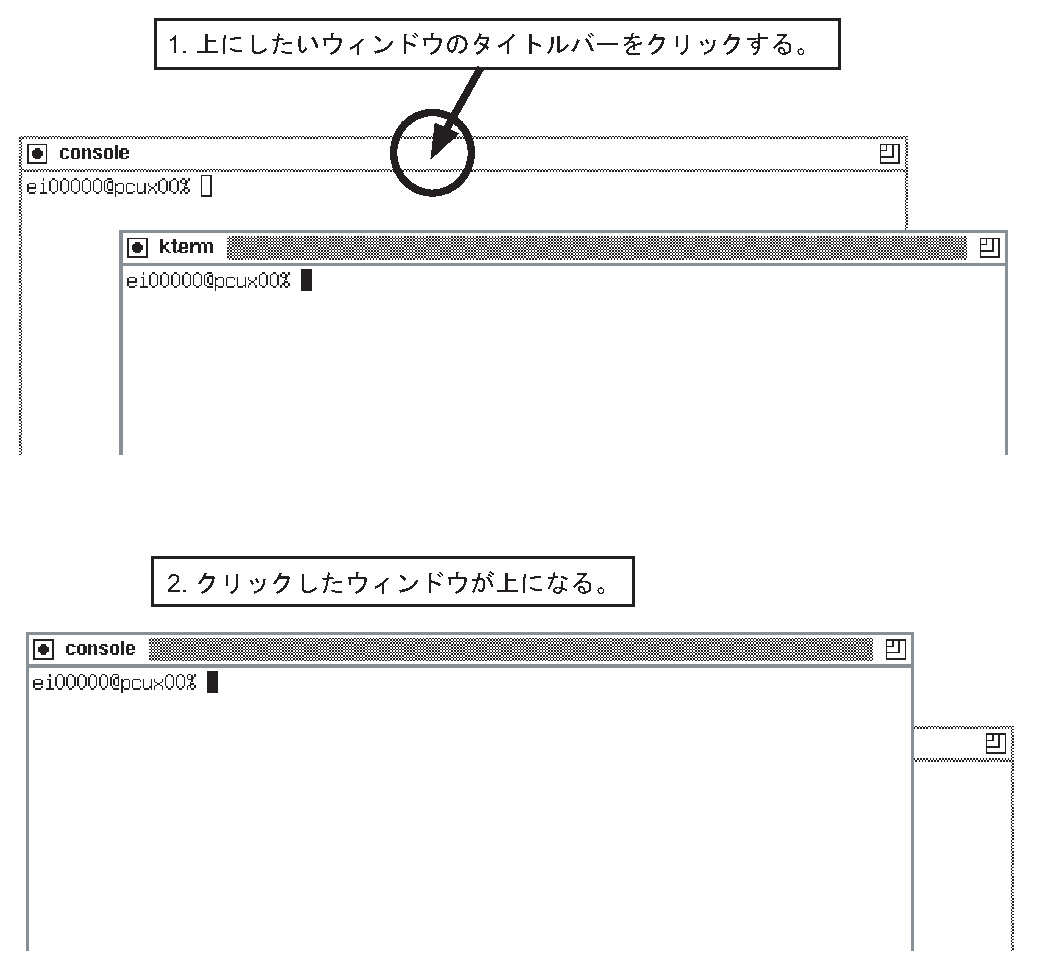
\includegraphics[scale=0.7]{raise.eps}}
\end{figure}

\newpage

\subsubsection{ウィンドウ・マネージャのメニューを使う}

何もないところで \KEYTOP{ボタン 1} を押して、Twm のメニューを出し、
その中の「Modify」から「Raize」を選ぶ。
マウス・カーソルが「●」になるので、これで上にしたいウィンドウをクリックする。

\begin{figure}[H]
\centering{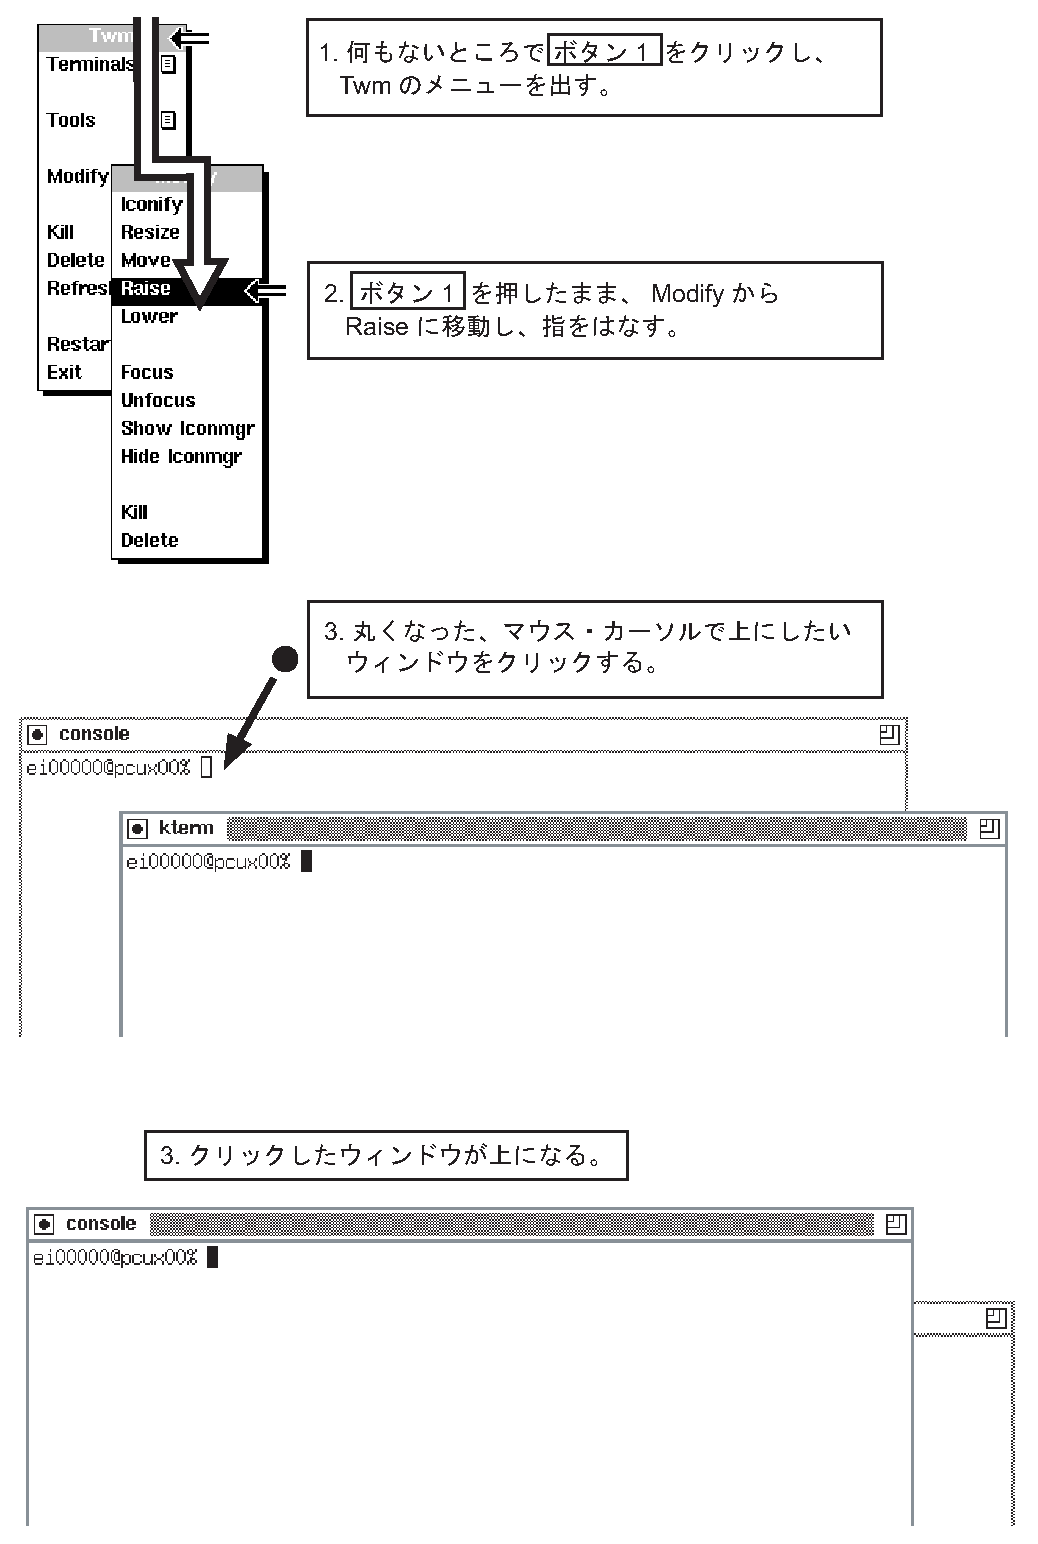
\includegraphics[scale=0.7]{raise02.eps}}
\end{figure}

\newpage
{~}
